\documentclass[11pt,a4paper]{article}
\usepackage{graphicx}
\usepackage{xcolor}
\usepackage{booktabs}
\usepackage{tabularx}
\usepackage{enumitem}
\usepackage{setspace}
\usepackage{hyperref}
\usepackage{multicol}
\usepackage{caption}

\definecolor{navyblue}{HTML}{003566}

\begin{document}

%  COVER PAGE
\thispagestyle{empty}
\noindent
\includegraphics[width=\textwidth]{cover_page-1.png}

\newpage

\section{Background}
Over the last few years, the Government of Madhya Pradesh has invested heavily in digital infrastructure through agencies like MAP-IT and NIC. This has led to a major rollout of digital platforms across the state’s key departments. 

Platforms like the Education Portal 3.0 or HRMIS are massive, but while the system is there, how much it’s actually used in a block-level office is often a different story. Even with all these platforms, what we see in local offices is that workflows still often run on paper registers and informal WhatsApp groups. It’s not that the tech is bad, but there’s a clear gap between what a system is built to do and the actual reality of how an official works on the ground.

\section{Rationale}
Getting officials to use these tools properly isn’t just about modernizing—it’s about making the state bureaucracy actually work faster. Right now, a huge chunk of IT budgets goes just into keeping legacy systems "alive" rather than making things more efficient. If we can bridge this gap, we can cut down the time officials spend on manual document processing that hasn’t really changed in decades.

\section{Capacity Building Framework}
Mission Karmayogi has changed how training works in the government, moving away from just learning basic rules to actual "role-based" skills. Since AIGGPA is the main training institute for the state, this research will help us design better, more practical IT training modules.

\section{Theoretical Framework}
To understand why some officials avoid these tools while others use them, this study uses the Unified Theory of Acceptance and Use of Technology (UTAUT). We’ll be looking at Performance Expectancy, Effort Expectancy, Social Influence, and Facilitating Conditions.

\vspace{0.5cm}
\begin{center}
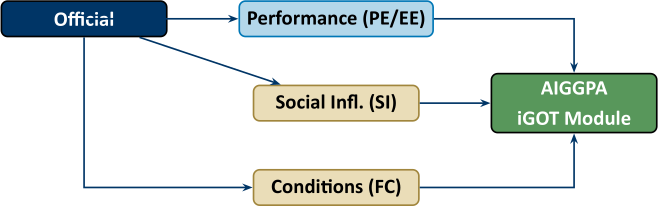
\includegraphics[width=0.8\textwidth]{figure_utaut.png}
\caption*{Figure 1. Mapping hurdles to AIGGPA interventions.}
\end{center}

\section{Research Objectives}
\begin{itemize}
  \item Identify which tools officials actually use for daily tasks (including informal tools).
  \item Track document flow to see where files still revert to paper.
  \item Capture IT department’s view on low-adoption areas.
  \item Categorize every hurdle under the UTAUT framework.
  \item Provide AIGGPA with a clear set of priority areas for training fixes.
\end{itemize}

\section{Scope}
\begin{itemize}
  \item \textbf{Departments:} School Education, Health, and Forest.
  \item \textbf{Respondents:} Class I, II, and III officials and IT staff.
  \item \textbf{Location:} Bhopal and selected district-level branches.
\end{itemize}

\section{Methodology}
We’re using a mixed-methods approach, combining hard numbers (login stats) with actual conversations with the people who use the software.

\subsection{Sampling Strategy}
A sample of 54 people picked across three departments and different ranks to get a good cross-section. 

\subsection{Data Collection}
1. Short, 30-minute sit-downs (interviews) in Hindi or English.
2. Anonymized login statistics from the IT nodal officers.
3. Desk Observation checklists to see the real facilitating conditions.

\subsection{Analysis Plan}
Everything we hear and see will be coded manually using ATLAS.ti to ensure we don't lose the nuance of government work. Once the tags are in, we’ll build our Gap Matrix to show exactly where the training is needed.

\section{Work Plan}
A 10-week cycle covering literature review, pilot testing, fieldwork (Weeks 4-8), and final report generation (Week 10).

\section{Budget}
Estimated at 30,000 INR, covering transit, software licenses, and field incidentals.

\section{Limitations and Ethics}
Covers access constraints and self-reporting bias. Participation is voluntary and anonymous, and no real names will be used in the report.

\section{What you'll get}
\begin{center}
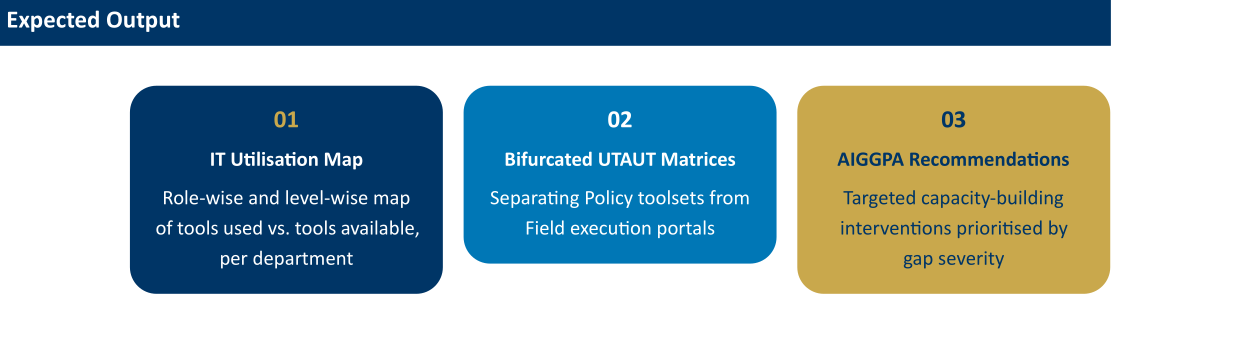
\includegraphics[width=0.9\textwidth]{expected_outputs.png}
\end{center}

\section{References}
Venkatesh, V., et al. (2003). User acceptance of technology.
Braun & Clarke (2006). Thematic analysis in psychology.
Heeks, R. (2003). Design-reality gaps in e-government.

\end{document}
